% System-level design consolidating the existing architecture diagram.
\section{System Architecture}
\label{sec:system-architecture}

The proposed platform uses a layered, modular architecture. The Flutter
Photographer App and the React web portals are presentation clients. They
communicate with the Backend API through authenticated HTTPS requests. The
backend owns business rules and access decisions; client-side role selectors
are interface demonstrations and must not be treated as authorization.

\begin{figure}[htbp]
\centering
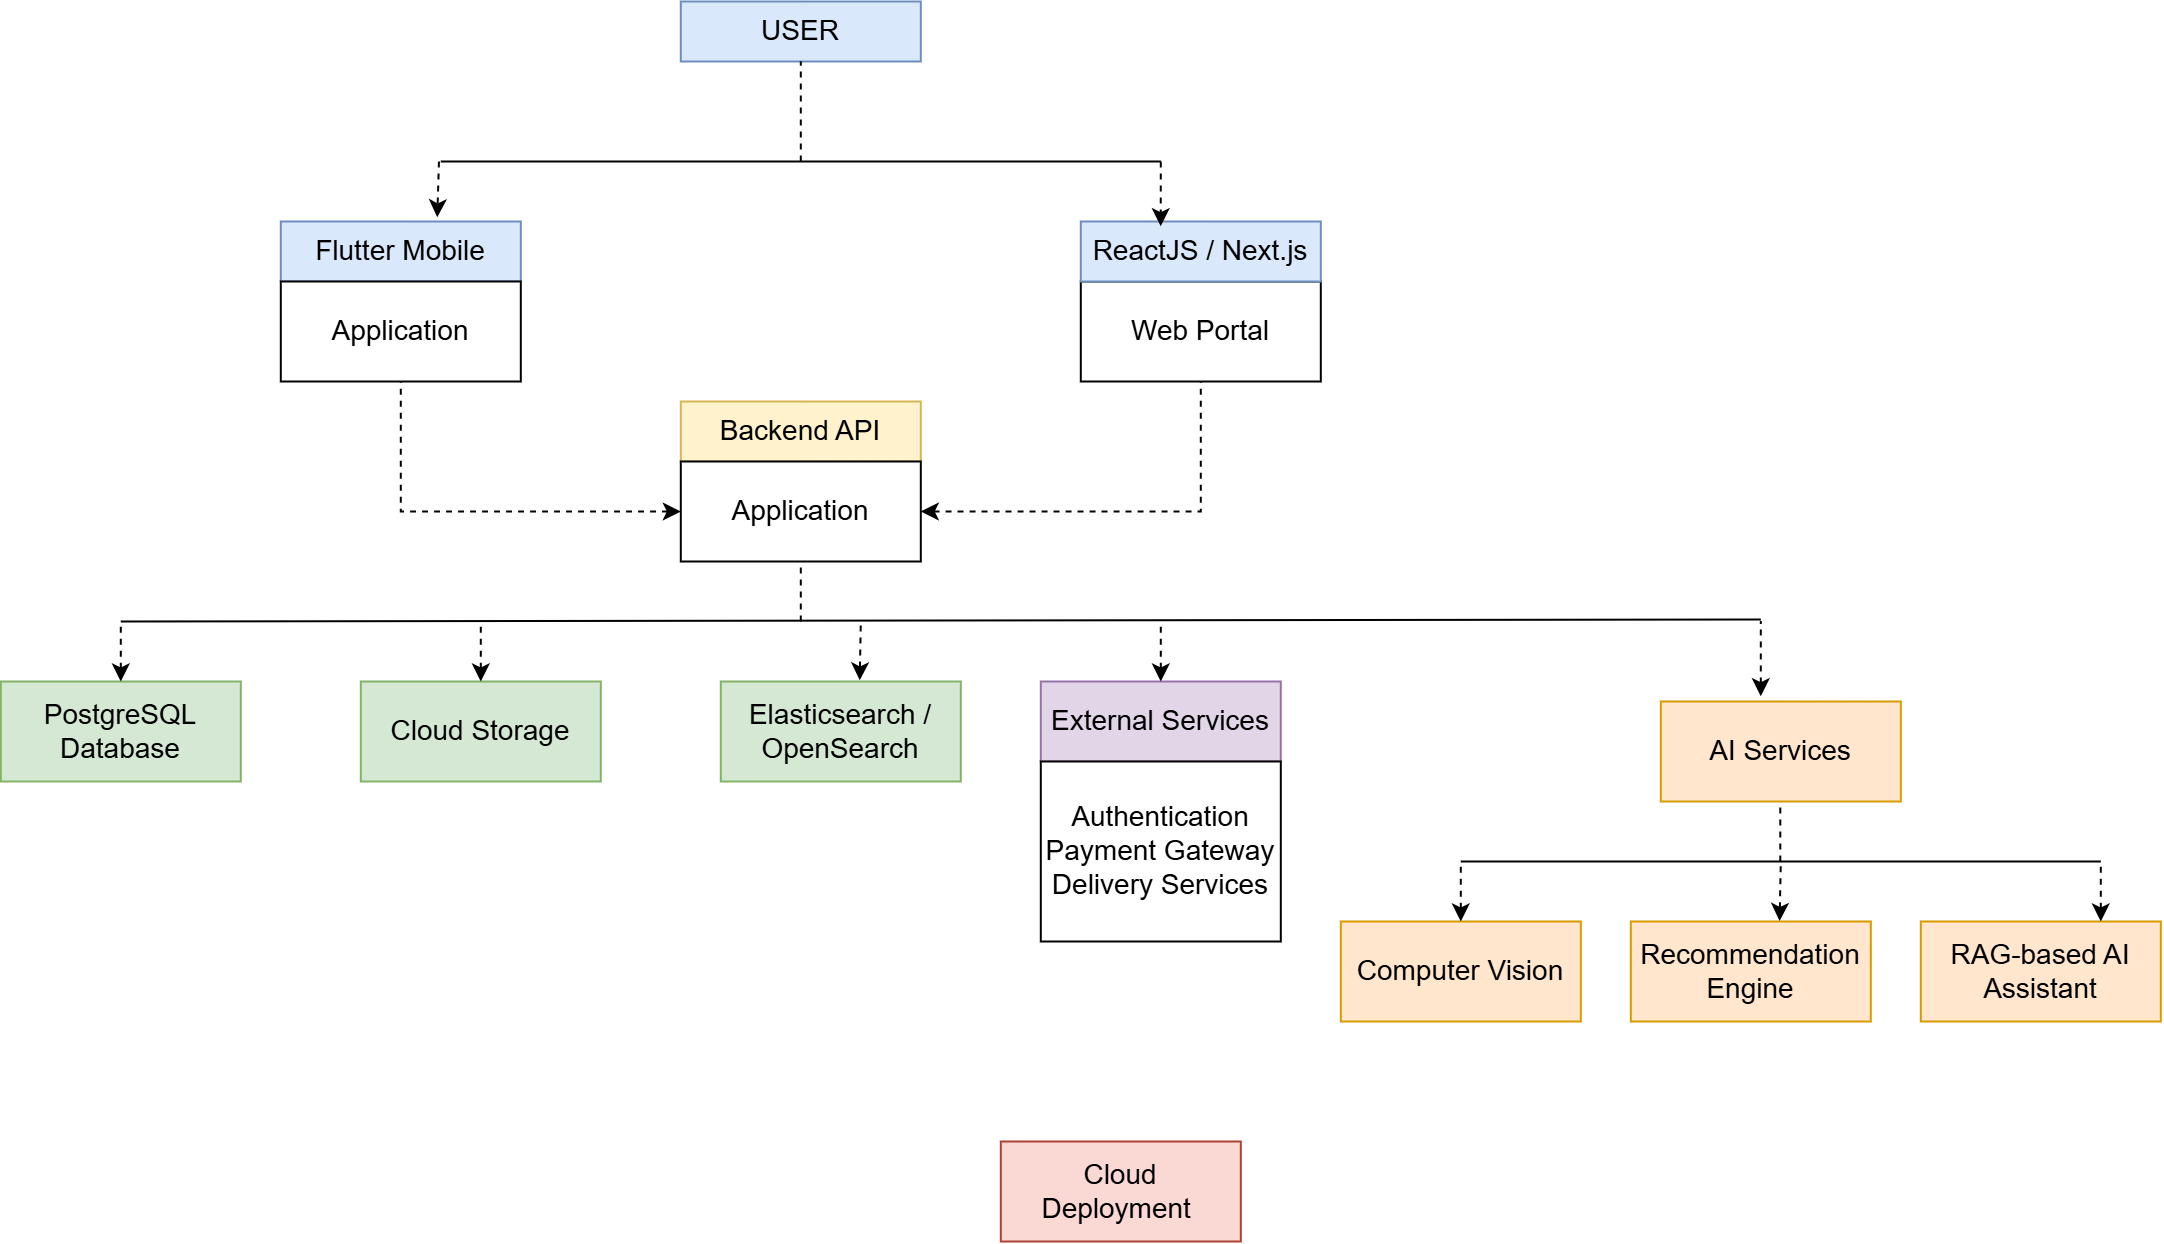
\includegraphics[width=\textwidth,height=0.56\textheight,keepaspectratio]{sections/08-system-architecture.png}
\caption{Proposed system architecture: shared API, data, storage, search, and AI services}
\label{fig:system-architecture}
\end{figure}

\subsection{Component Responsibilities}
\begin{description}[style=nextline]
\item[Client applications] Present discovery, booking, tracking, archive,
marketplace, and administration screens. Validate input for usability and show
loading, empty, and failure states. The API repeats all security-sensitive
validation independently.
\item[Backend API] Authenticate users, enforce role and resource ownership,
validate prices and services, manage the order lifecycle, and record audit
events. PostgreSQL transactions protect related state changes.
\item[PostgreSQL] Store accounts, labs, services, orders, workflow history,
and media metadata. Foreign keys and indexes support consistency and searches.
\item[Object storage] Store original scan files separately from relational
records. Access is private by default; authorized, short-lived links provide
downloads after ownership and order checks.
\item[AI service] Rank labs, retrieve domain knowledge, answer grounded
questions, and analyze scan quality. A backend adapter isolates this service
from public clients and prevents external model keys from reaching browsers.
\item[Search and external adapters] Search indexes, payment providers, and
logistics providers are proposed integration boundaries. They require
independent credentials, failure handling, and contract tests.
\end{description}

\subsection{Core Data Flow and Failure Handling}
A booking request contains selected lab/service identifiers and film details.
The backend validates ownership and availability, derives the charge from the
service catalogue, stores the order, and returns its identifier. Lab staff
advance only allowed status transitions. The status event and current order
state are committed together so a retry cannot silently duplicate a business
event.

For delivery, staff upload a validated file, attach metadata to the correct
order, and publish it after quality checking. The photographer sees only scans
belonging to an authorized order. Failed or incomplete uploads stay unpublished.
Payment and logistics callbacks must be authenticated and idempotent before
they change order state. If the AI service is unavailable, ordinary discovery
and order processing remain usable.

\subsection{Current Repository Boundary}
The diagram is the target design. The current repository implements clients
under \path{apps/}, an Express service under \path{backend/}, and Python AI
modules under \path{ai_service/}. The AI prototype uses local recommendation
data, TF--IDF retrieval, an extractive assistant, and image-quality heuristics.
It does not establish a deployed GPT integration or trained computer-vision
model. The frontend prototypes remain demonstrations until shared backend,
identity, storage, and notification contracts are connected and tested.
